\documentclass[article,36pt,extrafontsizes,oneside,openany,oldfontcommands]{memoir}
% \usepackage{natbib}
% \bibliographystyle{/Users/kengchichang/Dropbox/BibDesk/bst/econ_aer}
\usepackage[backend=biber,
    loccittracker=true,
    abbreviate=false,
    citetracker=false,
    authordate,
    sorting=ynt,
    isbn=false,
    hyperref=true,
    url=true,
    doi=true,
    eprint=false,
    hyperref=true,
    sortcites=true]{biblatex-chicago}
\addbibresource{/Users/kengchichang/Dropbox/Zotero/bib/all_papers_zotero.bib}
\AtBeginBibliography{\small}
\setlength{\bibitemsep}{0.0pt}
\setlength{\bibhang}{0.0pt}

\usepackage[export]{adjustbox}
\usepackage{wrapfig}

\usepackage{graphicx}
    \graphicspath{{figure/}}
\usepackage{amsmath, amsfonts, amssymb, amsthm}
\usepackage{mathtools}
\usepackage[charter,expert]{mathdesign}
\usepackage{fontspec}
\usepackage{xltxtra, xunicode}
\usepackage[utf8]{inputenc}
\RequirePackage[CJKmath = true, 
                indentfirst = false, 
                PunctStyle = {quanjiao}, 
                CheckSingle = true, 
                SlantFont, 
                BoldFont]
                {xeCJK}
%\usepackage{lmodern}
%\usepackage{times}
%\usepackage{mathptmx}
%\usepackage[minionint, lf, mathtabular]{MinionPro}
\usepackage{bm}
\RequirePackage{lipsum}
\RequirePackage{blindtext}
\RequirePackage[svgnames,table]{xcolor}
\RequirePackage{tikz}
\RequirePackage[framemethod=tikz]{mdframed}
\RequirePackage{color}
\RequirePackage{geometry}
\RequirePackage{adjmulticol}
\RequirePackage[skins,most,listings,skins]{tcolorbox}

%For kable extra package :)
\RequirePackage{longtable}
\RequirePackage{array}
\RequirePackage{multirow}
\RequirePackage{wrapfig}
\RequirePackage{float}
\RequirePackage{colortbl}
\RequirePackage{pdflscape}
\RequirePackage{pagecolor}
\RequirePackage{tabu}
\RequirePackage{threeparttablex}
\RequirePackage[normalem]{ulem}
\RequirePackage{makecell}
\RequirePackage{wrapfig}
\usepackage{xmpmulti, booktabs, multicol}
\usepackage{threeparttable}
\usepackage{dcolumn}
\newcolumntype{.}[1]{D{.}{.}{#1}}
\newcolumntype{,}[1]{D{,}{,}{#1}}
\usepackage{siunitx}
\sisetup{%
  mode = math,
  detect-all,  
  output-decimal-marker = {.},
  group-separator = {,},
  math-rm = \rmnumeric,
  text-rm = \rmnumeric,
}

%rof hyperrefs
\usepackage{color}
    \definecolor{MyBrown}{HTML}{3D3D00}
    \definecolor{MyBlue}{HTML}{003A75}  
    \definecolor{MyRed}{HTML}{6F1A2F}
    \definecolor{MyGreen}{HTML}{004847}
\usepackage{hyperref}
    \hypersetup{bookmarks = true,
                bookmarksnumbered = true,
                colorlinks = true,
                linkcolor = MyRed,
                citecolor = MyBlue, % hyperref is in conflict with natbib
                filecolor = MyBrown,
                urlcolor = MyGreen}
%For figure and table placement
\RequirePackage{float}
\floatplacement{figure}{H}
\floatplacement{table}{H}

%%%%%%%%% COLOURS %%%%%%%%
%Fill/ Line Colours
\definecolor{titleboxbgcol}{HTML}{ec6408}
\definecolor{titleboxbordercol}{HTML}{205DA4}
\definecolor{columnlinecol}{HTML}{008080}
\definecolor{bodybgcol}{HTML}{ffffff}
\definecolor{sectitlebgcol}{HTML}{ec6408}
\definecolor{sectitlebordercol}{HTML}{ec6408}
% Text Colours
\definecolor{titletextcol}{HTML}{FFFFFF}
\definecolor{authortextcol}{HTML}{FFFFFF}
\definecolor{affiliationtextcol}{HTML}{000000}
\definecolor{sectitletextcol}{HTML}{FFFFFF}
\definecolor{bodytextcol}{HTML}{000000}
\definecolor{footnotetextcol}{HTML}{000000}
\definecolor{citecol}{HTML}{CC0000}
\definecolor{urlcol}{HTML}{008080}
\definecolor{linkcol}{HTML}{008080}


%Memoir spacing options
%spacing between figure/ table and caption
\setlength{\abovecaptionskip}{0.4in}
\setlength{\belowcaptionskip}{0.2in}
\captionnamefont{\normalsize}
\captiontitlefont{\normalsize}

%define column options
\setlength{\columnseprule}{0pt}
\def\columnseprulecolor{\color{columnlinecol}}

%define section title features
\setsubsubsecheadstyle{\small\color{sectitletextcol}\textbf}% Set \section style
\setsecnumformat{}
\def\sectionmark#1{\markboth{#1}{#1}}

%%%%%%%%%%%% TCOLORBOXES TO THE RESCUE %%%%%%%%%%%%%%%%%%%%
%Title Box
\newtcolorbox{topbox}{
enhanced,
colback=titleboxbgcol,
colframe=titleboxbordercol,
halign=center,
boxrule=0cm,
sharp corners=all,
 overlay={
    % \node[anchor=south west]
    %   at ([xshift=1in,yshift=1in]frame.south west)
    %    {\includegraphics[width=3in]{Figures/posterdownlogo}};
    % \node[anchor=south east]
    %   at ([xshift=-1in,yshift=1in]frame.south east)
    %    {\includegraphics[width=3in]{Figures/posterdownlogo}};
       }

}
%Body Section Title Box
\newtcolorbox{myboxstuff}[1][]{
code={\parindent=0em},
colframe=sectitlebordercol,
nobeforeafter,
left skip=0pt,
valign=center,
halign=center,
fontupper=\large\bfseries,
colupper=sectitletextcol,
boxrule=2mm,
colback=sectitlebgcol,
sharp corners=south, #1}
\newcommand{\mybox}[1]{%
\begin{myboxstuff}
\strut #1
\end{myboxstuff}%
}
\makeheadstyles{MyBox}{
    \setsecheadstyle{\mybox}
}
\headstyles{MyBox}\makepagestyle{MyBox}
%-----------------------------------------------------
%Make sure that the page is empty of any preset items from memoir
\thispagestyle{empty}

%biblatex options
%\usepackage{natbib}
%\DeclareTextCommandDefault{\nobreakspace}{\leavevmode\nobreak\ } % AER style nobreak
\renewcommand{\bibname}{\hrule}
%\renewcommand{\bibsection}{}
%\renewcommand*{\bibfont}{\fontsize{40pt}{45pt}\selectfont}
%\setlength{\bibsep}{0pt plus 0.3ex}

%Remove section numbering & set 2nd level header as first level
%to avoid the automatic new page generated from memoir chapter
%formatting
\counterwithout{section}{chapter}
\makechapterstyle{mydefault}{
\addtocounter{secnumdepth}{2}
\setsecheadstyle{\mybox}
\setsubsecheadstyle{\itshape}
\setsubsubsecheadstyle{\itshape}
}

%set the chapterstyle
\chapterstyle{mydefault}

%define column spacing
\setlength\columnsep{0.5in}

%spacing params
\setlength\parindent{0em}
\setlength\parskip{0em}
\setlength\hangparas{0em}

%spacing after section head title
\setaftersecskip{0em}
\setbeforesecskip{0.5em}
\setlength\textfloatsep{0in} % distance between floats on the top or the bottom and the text
\setlength\floatsep{0.1in} % distance between two floats
\setlength\intextsep{0.5in} % distance between floats inserted inside the page text (using h) and the text proper
\makeatletter
\g@addto@macro{\normalsize}{%
%    \setlength\abovedisplayskip{30pt} % spacing above equations
%    \setlength\abovedisplayshortskip{15pt} % spacing immediately above equations
%    \setlength\belowdisplayskip{0pt} % spacing below equations
%    \setlength\belowdisplayshortskip{0pt} % spacing immediately below equations
%    \setlength{\displayindent}{0in}
%    \setlength{\predisplaysize}{0in}
    } 
\makeatother

\setstocksize{36in}{48in}
\settrimmedsize{\stockheight}{\stockwidth}{*}
\settypeblocksize{36in}{48in}{*}
\setlrmargins{*}{*}{1}
\setulmarginsandblock{2.5cm}{0cm}{*}
\setmarginnotes{0em}{0cm}{0cm}
\setlength{\footskip}{0cm}
\setlength{\footnotesep}{0cm}
\setlength{\headheight}{0pt}
\setlength{\headsep}{0pt}
\setlength{\trimtop}{0pt}
\setlength{\trimedge}{0pt}
\setlength{\uppermargin}{0pt}
\checkandfixthelayout
\usepackage{enumitem}
\usepackage{bbm}
\usepackage{dsfont}
\def\one{\mathrm{1}\hspace{-12pt}\mathrm{1}}
\setlist[enumerate]{topsep=0pt,itemsep=-1ex,partopsep=1ex,parsep=1ex,leftmargin=2ex}
\setlist[itemize]{topsep=0pt,itemsep=-1ex,partopsep=1ex,parsep=1ex,leftmargin=2ex}

%Footnote to white
\RequirePackage{footmisc}
\def\footnotelayout{\centering\color{footnotetextcol}}

% see https://stackoverflow.com/a/47122900
\usepackage{color}
\usepackage{fancyvrb}
\newcommand{\VerbBar}{|}
\newcommand{\VERB}{\Verb[commandchars=\\\{\}]}
\DefineVerbatimEnvironment{Highlighting}{Verbatim}{commandchars=\\\{\}}
% Add ',fontsize=\small' for more characters per line
\usepackage{framed}
\definecolor{shadecolor}{RGB}{248,248,248}
\newenvironment{Shaded}{\begin{snugshade}}{\end{snugshade}}
\newcommand{\AlertTok}[1]{\textcolor[rgb]{0.94,0.16,0.16}{#1}}
\newcommand{\AnnotationTok}[1]{\textcolor[rgb]{0.56,0.35,0.01}{\textbf{\textit{#1}}}}
\newcommand{\AttributeTok}[1]{\textcolor[rgb]{0.77,0.63,0.00}{#1}}
\newcommand{\BaseNTok}[1]{\textcolor[rgb]{0.00,0.00,0.81}{#1}}
\newcommand{\BuiltInTok}[1]{#1}
\newcommand{\CharTok}[1]{\textcolor[rgb]{0.31,0.60,0.02}{#1}}
\newcommand{\CommentTok}[1]{\textcolor[rgb]{0.56,0.35,0.01}{\textit{#1}}}
\newcommand{\CommentVarTok}[1]{\textcolor[rgb]{0.56,0.35,0.01}{\textbf{\textit{#1}}}}
\newcommand{\ConstantTok}[1]{\textcolor[rgb]{0.00,0.00,0.00}{#1}}
\newcommand{\ControlFlowTok}[1]{\textcolor[rgb]{0.13,0.29,0.53}{\textbf{#1}}}
\newcommand{\DataTypeTok}[1]{\textcolor[rgb]{0.13,0.29,0.53}{#1}}
\newcommand{\DecValTok}[1]{\textcolor[rgb]{0.00,0.00,0.81}{#1}}
\newcommand{\DocumentationTok}[1]{\textcolor[rgb]{0.56,0.35,0.01}{\textbf{\textit{#1}}}}
\newcommand{\ErrorTok}[1]{\textcolor[rgb]{0.64,0.00,0.00}{\textbf{#1}}}
\newcommand{\ExtensionTok}[1]{#1}
\newcommand{\FloatTok}[1]{\textcolor[rgb]{0.00,0.00,0.81}{#1}}
\newcommand{\FunctionTok}[1]{\textcolor[rgb]{0.00,0.00,0.00}{#1}}
\newcommand{\ImportTok}[1]{#1}
\newcommand{\InformationTok}[1]{\textcolor[rgb]{0.56,0.35,0.01}{\textbf{\textit{#1}}}}
\newcommand{\KeywordTok}[1]{\textcolor[rgb]{0.13,0.29,0.53}{\textbf{#1}}}
\newcommand{\NormalTok}[1]{#1}
\newcommand{\OperatorTok}[1]{\textcolor[rgb]{0.81,0.36,0.00}{\textbf{#1}}}
\newcommand{\OtherTok}[1]{\textcolor[rgb]{0.56,0.35,0.01}{#1}}
\newcommand{\PreprocessorTok}[1]{\textcolor[rgb]{0.56,0.35,0.01}{\textit{#1}}}
\newcommand{\RegionMarkerTok}[1]{#1}
\newcommand{\SpecialCharTok}[1]{\textcolor[rgb]{0.00,0.00,0.00}{#1}}
\newcommand{\SpecialStringTok}[1]{\textcolor[rgb]{0.31,0.60,0.02}{#1}}
\newcommand{\StringTok}[1]{\textcolor[rgb]{0.31,0.60,0.02}{#1}}
\newcommand{\VariableTok}[1]{\textcolor[rgb]{0.00,0.00,0.00}{#1}}
\newcommand{\VerbatimStringTok}[1]{\textcolor[rgb]{0.31,0.60,0.02}{#1}}
\newcommand{\WarningTok}[1]{\textcolor[rgb]{0.56,0.35,0.01}{\textbf{\textit{#1}}}}

% choose font family
\RequirePackage{etoolbox}
%\RequirePackage{unicode-math}
\defaultfontfeatures{Ligatures=TeX,Scale=MatchLowercase,Mapping=tex-text]}
\setsansfont{Times New Roman}
\setmainfont{Times New Roman}
%\setmathfont{Fira Math}
\setmonofont[Scale=0.85]{Times New Roman}
\newfontfamily\compthick{Times New Roman}
\newfontfamily\compthin{Times New Roman}
\newfontfamily\comp{Times New Roman}
\newfontfamily\thin{Times New Roman}
%\setCJKmainfont[BoldFont={Times New Roman}]{Times New Roman}
%\setCJKsansfont[BoldFont={Times New Roman}]{Times New Roman}
%\setCJKmonofont[BoldFont={Times New Roman}]{Times New Roman}

% define the BODYBGCOL
\newpagecolor{bodybgcol}

%sets footnote to be white hopefully
\renewcommand\footnoterule{}
\renewcommand{\thempfootnote}{\footnotesize\color{footnotetextcol}{\arabic{mpfootnote}}}

%include arbitrary input from header-includes field
%\usepackage[font={footnotesize, it}]{caption}
%-------------- Begin Document -------------------%
\begin{document}

%-------------- Title Box Start ------------------%
%tcolorbox allows for pictures hopefully
\begin{topbox}
  \color{titletextcol}
  \vspace{0.8in}
  \bfseries
  \fontsize{100pt}{100pt}\selectfont
  {Graph-Based~~Deep~~Learning~~for~~Fraud~~Detection~~in~~ETH~~Transaction~~Networks}\\[0.5in]  %% SC
  \color{authortextcol} 
  \mdseries
  \fontsize{40pt}{40pt}\selectfont
  {Stephen Gelinas~~$\cdot$~~\texttt{sgelinas@ucsd.edu}~~$\cdot$~~Kazuma Yamamoto~~$\cdot$~~\texttt{kayamamo@ucsd.edu}~~$\cdot$~~Ethan Zhou~~$\cdot$~~\texttt{ezhou@ucsd.edu}} 
  % \\[0.2in] %% SC
  % \color{affiliationtextcol} \large{UC San Diego} %% SC
  %\includegraphics[width=0.1\linewidth]{figure/tg_logo_full.png}
  \vspace{0.6in}
\end{topbox}


%--------------- Title Box End -------------------%
%----------------- Body Start --------------------%
% Begin body of poster


\fontsize{40pt}{40pt}\selectfont

\begin{adjmulticols*}{3}{0.5in}{0.5in}
\color{bodytextcol}

\section{Background \& Research Question}

\begin{adjustwidth}{0in}{0in}
\begin{itemize}[topsep=0pt,itemsep=0ex,partopsep=0ex,parsep=0ex]
\item According to the FTC, cryptocurrency scams have cost online users over \$1 Billion since 2021.
\item With access to Ethereum transaction networks, we can model and train phishing detection as a node classification problem.
\item How do non-graph supervised learning algorithms compare to graph-based deep learning approaches for fraud detection? 
\end{itemize}
\end{adjustwidth}


\section{Why Graph?}

\begin{adjustwidth}{0in}{0in}
\begin{itemize}[topsep=0pt,itemsep=0ex,partopsep=0ex,parsep=0ex]
\item Graph algorithms can numerically represent information that is inherent to a network.
\item Graph neural networks take advantage of learning the structural information within a graph and embedding information about neighboring nodes in the network.
\item This allows for graph models to heavily outperform traditional learning algorithms.

%\item 26K authentic memes from \texttt{r/meme} subreddit (authentic memes)
%\item 15K non-meme image-with-text data (COCO-Text) as negative sample for training (so not simply a classifier for images with or without text)
%\item 26K images from IRA on Twitter (coordinated memes if classified as meme)
\end{itemize} 
\end{adjustwidth}


\section{Data Source}
\begin{adjustwidth}{0.1in}{0in}
%\begin{itemize}[topsep=0pt,itemsep=0ex,partopsep=0ex,parsep=0ex]
The \href{http://xblock.pro/#/dataset/6}{XBlock} dataset containing transactions of 890 Ethereum accounts
\begin{enumerate}[topsep=0pt,itemsep=0ex,partopsep=0ex,parsep=0ex]
\item Collect subgraphs by K-order sampling with K-in = 1, K-out = 3 for each of the 890 objective nodes 
\item Splice into a large-scale network with 86,623 nodes and 106,083 edges
\begin{figure}
	\centering
	\includegraphics[width=.8\linewidth]{figure/k-order_sampling.png}
	\caption{How our data was sourced}
\end{figure}
\linebreak
On the figure above, based on the assumption that a typical money transfer flow is centered on a phishing node, the previous node of the phishing node may be a victim, and the next one to three nodes may be the bridge nodes with money laundering behaviors.

\end{enumerate}
%\item Classify IRA images into memes vs. non-memes (test accuracy $>0.97$)
%\item Extract visual embeddings jointly for both authentic memes (Reddit) and coordinated memes (IRA) using DeepCluster \href{http://arxiv.org/abs/1807.05520}{(Caron et al. 2019)}\\
%{\centering \includegraphics[width=.8\linewidth]{figure/filler.png}}
%\item Cluster memes based on visual embeddings using K-means 
%\item Label the clusters and compare between authentic/coordinated
\end{adjustwidth}
\section{Recent Advancements in the Field}
\begin{adjustwidth}{0.1in}{0in}
\begin{itemize}[topsep=0pt,itemsep=0ex,partopsep=0ex,parsep=0ex]
\item The field of graph data science is relatively new and very active, and key advancements happen very frequently
\item For example, all of the models we used were developed in the last several years. GCN and N2V are from 2016, GAT, GraphSage, and TA-GCN are from 2017.
\end{itemize} 
\end{adjustwidth}


\columnbreak
\begin{figure}
	\centering
	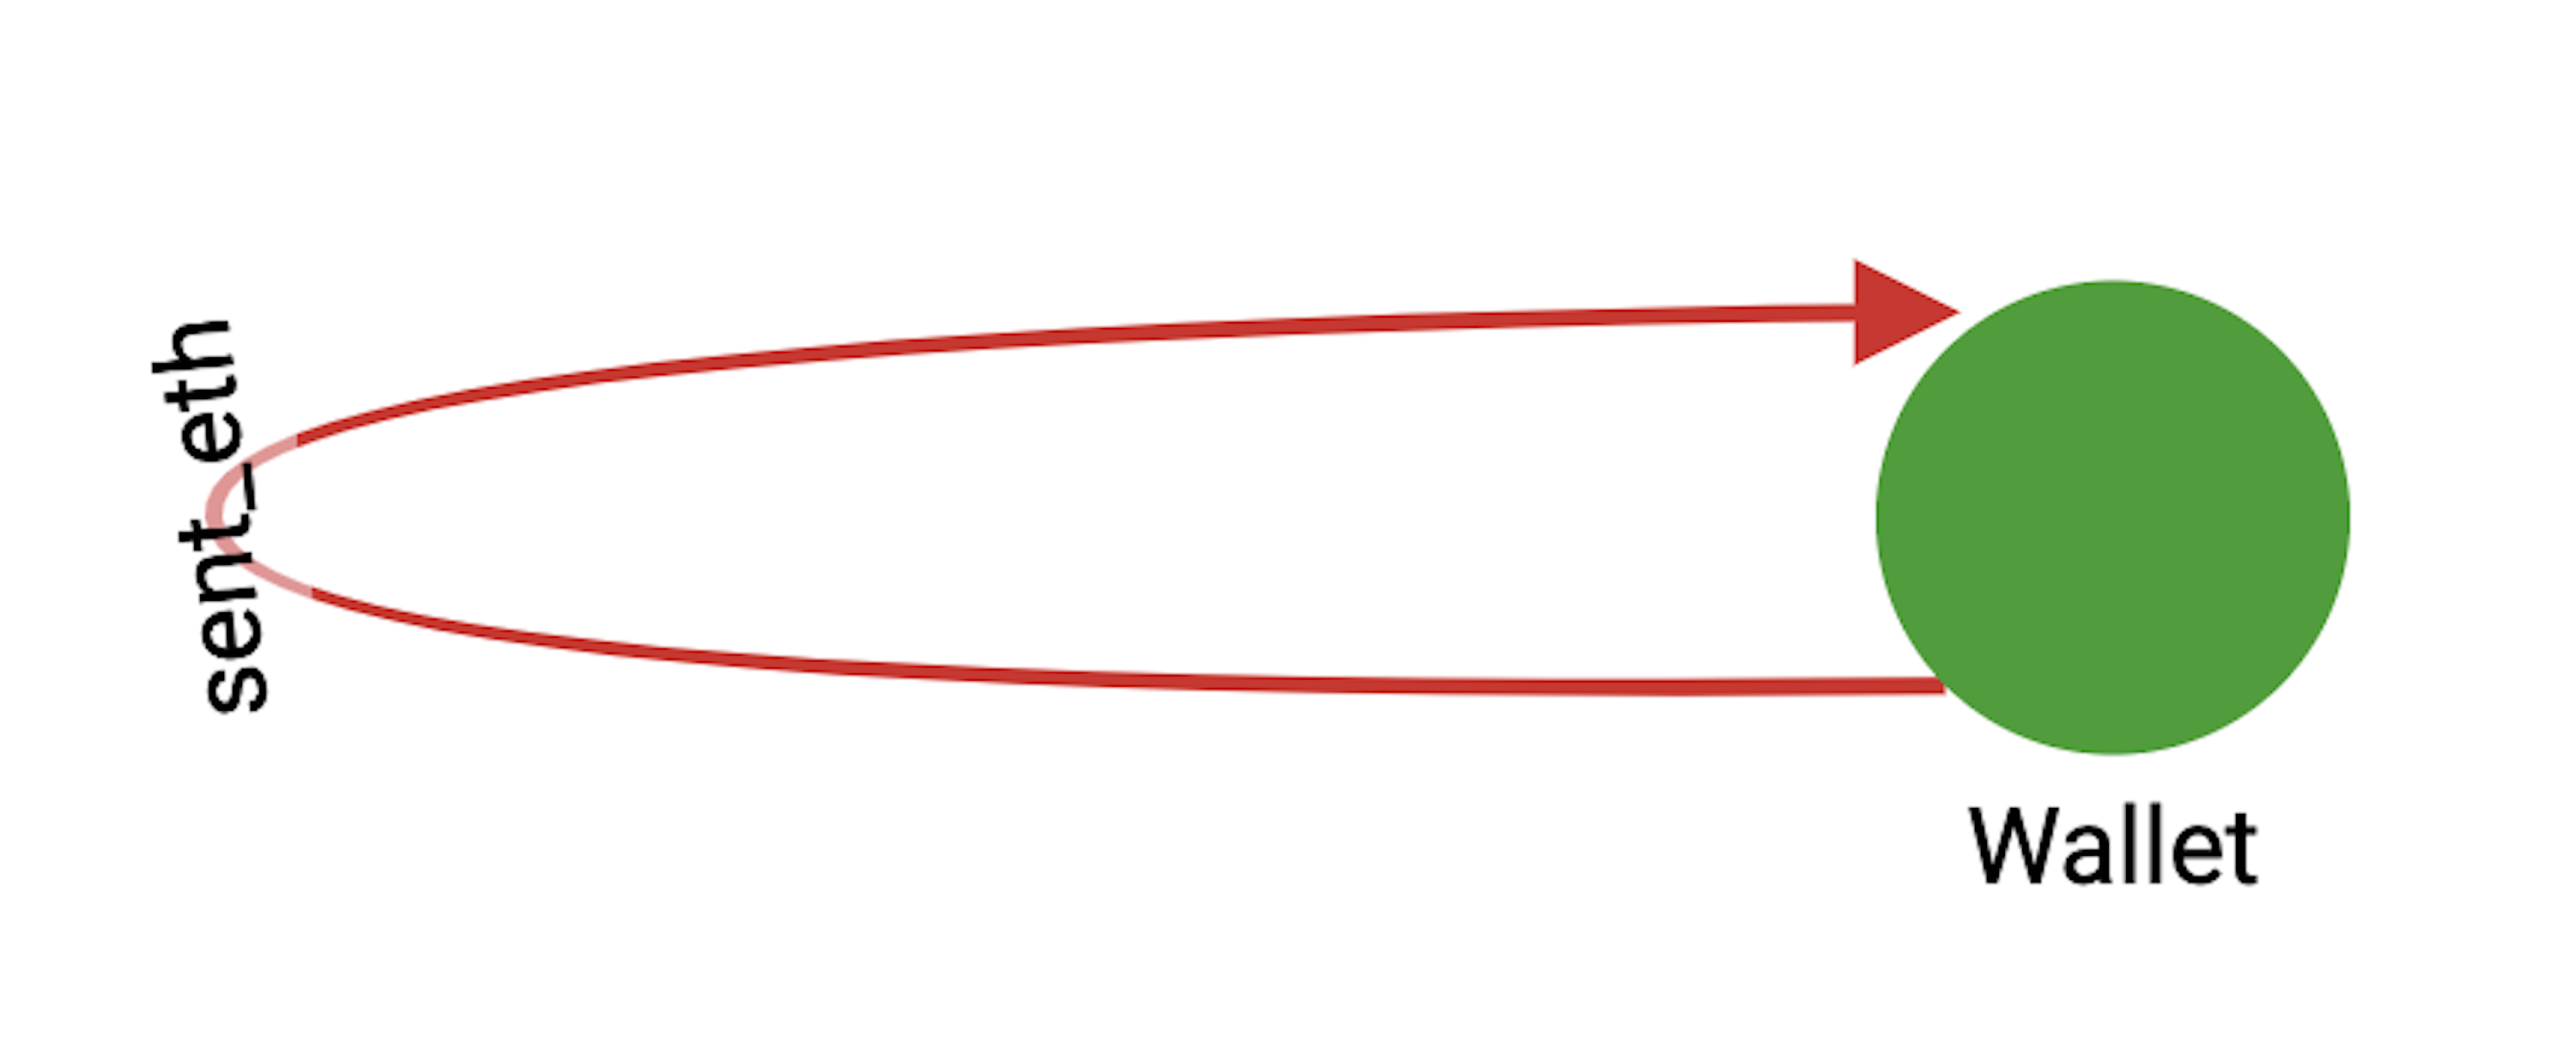
\includegraphics[width=0.8\linewidth]{figure/graph_schema.png}
	\caption{An example of how our graph schema looks, at the basic level}
\end{figure}
\linebreak
\begin{figure}
	\centering
	\includegraphics[width=0.65\linewidth]{figure/table_data.png}
	\caption{Performance of each model}
\end{figure}
\linebreak
\begin{figure}
	\centering
	\includegraphics[width=0.75\linewidth]{figure/fake_importance.png}
	\caption{The relative importance of each feature to our models}
\end{figure}
\columnbreak

\section{Methods Overview}
\begin{adjustwidth}{0.1in}{0in}
\begin{itemize}[topsep=0pt,itemsep=0ex,partopsep=0ex,parsep=0ex]
\item The transaction network is represented as a directed graph, where each node represents a wallet in the network, and each directed edge between wallets represents the transfer of currency.
\item Features are assigned to each node, including in-degree, out-degree, total transaction value, and more.
\item The fraud detection task is ran as a node classification problem, and the performance of the models will be evaluated.


%\item Classify IRA images into memes vs. non-memes (test accuracy $>0.97$)
%\item Extract visual embeddings jointly for both authentic memes (Reddit) and coordinated memes (IRA) using DeepCluster \href{http://arxiv.org/abs/1807.05520}{(Caron et al. 2019)}\\
%{\centering \includegraphics[width=.8\linewidth]{figure/filler.png}}
%\item Cluster memes based on visual embeddings using K-means 
%\item Label the clusters and compare between authentic/coordinated
\end{itemize} 
\end{adjustwidth}


\section{Conclusion and Summary of Findings}
\begin{adjustwidth}{0.1in}{0in}
\begin{itemize}[topsep=0pt,itemsep=0ex,partopsep=0ex,parsep=0ex]
\item Graph-based features improves overall model performance for both graph-based and non-graph-based models.
\item Graph neural networks, specifically TA-GCN, performed best in the fraud detection task, as GNNs are able to learn the networks’ structural information.
\item The most important features for predicting  fraudulent wallets are pagerank and the maximum amount of ETH sent between wallets.


%\item Latent visual embeddings reveal similarity between memes
%\item Authentic and coordinated memes share most visual themes
%\item Coordinated IRA memes more military, gender, quotes
%\item Authentic Reddit memes more movie characters, comics
%\item IRA accounts are not widely utilizing popular meme schemes in the US
%\item Logistic regression on visual embedding discern IRA with $F_1=0.84$
\end{itemize} 
\end{adjustwidth}

\section{References}
\begin{adjustwidth}{0.1in}{0in}
\begin{enumerate}[topsep=0pt,itemsep=0ex,partopsep=0ex,parsep=0ex]
\item Alin Deutsch, Yu Xu, Mingxi Wu, Victor Lee: “TigerGraph: A Native MPP Graph Database”, 2019; arXiv:1901.08248
\item Jiajing Wu, Qi Yuan, Dan Lin, Wei You, Weili Chen, Chuan Chen, Zibin Zheng: “Who Are the Phishers? Phishing Scam Detection on Ethereum via Network Embedding”, 2019, TSMC.2020.3016821; arXiv:1911.09259
\item Jiajing Wu, Dan Lin, Zibin Zheng, Qi Yuan: “T-EDGE: Temporal Weighted MultiDiGraph Embedding for Ethereum Transaction Network Analysis”, 2019, Front. Phys. 8:204 (2020); arXiv:1905.08038
\item Panpan Li, Yunyi Xie, Xinyao Xu, Jiajun Zhou, Qi Xuan: “Phishing Fraud Detection on Ethereum using Graph Neural Network”, 2022; arXiv:2204.08194
\item Jian Du, Shanghang Zhang, Guanhang Wu, Jose M. F. Moura, Soummya Kar: “Topology Adaptive Graph Convolutional Networks”, 2017; arXiv:1710.10370
\item Mark Cheung, John Shi, Lavender Yao Jiang, Oren Wright, José M. F. Moura: “Pooling in Graph Convolutional Neural Networks”, 2020; arXiv:2004.03519



%\item Latent visual embeddings reveal similarity between memes
%\item Authentic and coordinated memes share most visual themes
%\item Coordinated IRA memes more military, gender, quotes
%\item Authentic Reddit memes more movie characters, comics
%\item IRA accounts are not widely utilizing popular meme schemes in the US
%\item Logistic regression on visual embedding discern IRA with $F_1=0.84$
\end{enumerate} 
\end{adjustwidth}

\linebreak

\begin{figure}
	\centering
	\begin{minipage}{0.45\linewidth}
		\centering
		\includegraphics[width=0.6\linewidth]{figure/qrcode.png}
	\end{minipage}\hfill
	\begin{minipage}{0.45\linewidth}
		\centering
		
\includegraphics[width=0.9\linewidth]{figure/tigergraph_logo.png}
	\end{minipage}\hfill
\end{figure}

\begin{figure}
	\end{figure}
%\section{Example Clusters}
%\begin{adjustwidth}{0.1in}{0in}
%\begin{figure}
%    \includegraphics[width=\linewidth]{figure/filler.png}
%    \\[1cm]
 %   \includegraphics[width=\linewidth]{figure/filler.png}
%\end{figure}
%\vspace{-3cm}
%\end{adjustwidth}

%\columnbreak

% \begin{minipage}{.32\textwidth}
  %\begin{figure}
    %\vspace{2cm} \hspace{2.5cm} 
    %\includegraphics[width=1.25\linewidth]{figure/filler.png}
  %\end{figure}
% \end{minipage}


%\begin{adjustwidth}{0.1in}{0in}
%\vspace{1.25cm}
%\begin{figure}
   % \includegraphics[width=\linewidth]{figure/filler.png}
    %\\[1cm]
    %\includegraphics[width=\linewidth]{figure/filler.png}
%\end{figure}
%\vspace{-3cm}
%\end{adjustwidth}


%\columnbreak


% \begin{minipage}{.2\textwidth}
  %\begin{figure}
    %\centering
    %\hspace{2cm}
    %\includegraphics[width=.15\linewidth]{figure/filler.png}
    %Comments/feedbacks
    %\hspace{5cm}
    %\includegraphics[width=.63\linewidth]{figure/filler.png}
  %\end{figure}
% \end{minipage}




%\hrule
\printbibliography[heading=none]


\end{adjmulticols*}
%------------------ Body End ---------------------%
%end the poster

\end{document}

